%% CH14 COMPLEX NUMBERS EQ
\newcommand{\figTJCsq}{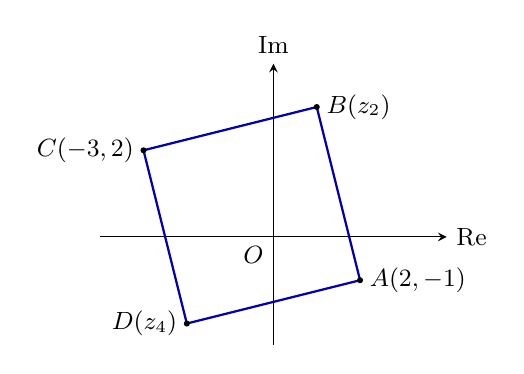
\begin{tikzpicture}[scale=0.55,font=\small,>=stealth]
\draw[->](-4,0)--(4,0)node[right]{Re};\draw[->](0,-2.5)--(0,4)node[above]{Im};\node[below left]at(0,0){$O$};
\draw[blue!70!black,thick](2,-1)--(1,3)--(-3,2)--(-2,-2)--cycle;
\fill(2,-1)circle(2pt)node[right]{$A(2,-1)$};\fill(1,3)circle(2pt)node[right]{$B(z_{2})$};
\fill(-3,2)circle(2pt)node[left]{$C(-3,2)$};\fill(-2,-2)circle(2pt)node[left]{$D(z_{4})$};
\end{tikzpicture}}
\newcommand{\figTJCac}{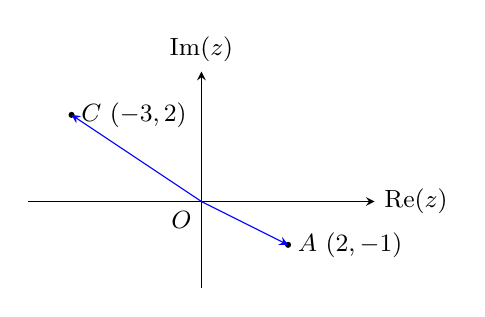
\begin{tikzpicture}[scale=0.55,font=\small,>=stealth]
\draw[->](-4,0)--(4,0)node[right]{Re$(z)$};\draw[->](0,-2)--(0,3)node[above]{Im$(z)$};\node[below left]at(0,0){$O$};
\fill(2,-1)circle(2pt)node[right]{$A\ (2,-1)$};\fill(-3,2)circle(2pt)node[right]{$C\ (-3,2)$};
\draw[->,blue](0,0)--(2,-1);\draw[->,blue](0,0)--(-3,2);
\end{tikzpicture}}
\newcommand{\figVJCa}[1]{\begin{tikzpicture}[scale=1.1,font=\small]
\draw[->](-1.6,0)--(1.6,0)node[right]{Re};\draw[->](0,-1.5)--(0,2.2)node[above]{Im};\node[below right]at(0,0){$O$};
\draw[dashed](0,0)--(-0.707,0.707)node[midway,below left]{$1$};\draw[dashed](0,0)--(-1.225,-1.225)node[midway,above left]{$\sqrt3$};
\draw[dashed](-0.707,0.707)--(0.518,1.932)node[midway,above left]{$\sqrt3$};#1
\node at(-0.707,0.707){$\times$};\node[left]at(-0.75,0.75){$P$};\node at(-1.225,-1.225){$\times$};\node[below]at(-1.225,-1.3){$Q$};
\node at(0.518,1.932){$\times$};\node[right]at(0.55,1.95){$R$};
\end{tikzpicture}}
%% ===== 141 TJC 2025 Prelim P1 Q8 (soln: TJC_2025_H2_Math_Prelim_P1_Solutions.pdf pp8-9)
\defQ{141}{}{%
\begin{qparts}
\pt{(a)} The complex numbers $z$ and $w$ satisfy the following equations.
\[2z+|w|=2-4\mathrm{i}\qquad\mathrm{i}z-w=2\mathrm{i}\]
Find $z$ and $w$, giving your answers in the form $a+\mathrm{i}b$, where $a$ and $b$ are real numbers. \mk{5}
\pt{(b)} It is given that $z_{1}=2-\mathrm{i}$ and $z_{3}=-3+2\mathrm{i}$. On an Argand diagram, mark the points $A$ and $C$ representing $z_{1}$ and $z_{3}$ respectively. \mk{1}\par
The points $B$ and $D$ on the Argand diagram represent complex numbers $z_{2}$ and $z_{4}$ respectively. Given that $ABCD$ is a square, labelled in an anti-clockwise direction, find $z_{2}$ and $z_{4}$. \mk{4}
\end{qparts}
\src{TJC 2025 Prelim P1 Q8}}
\defS{141}{%
\begin{gtpart}{(a)}{5}\begin{topalign}
2z+\left|w\right|&=2-4\mathrm{i}\quad\text{--- (1)}\\
\mathrm{i}z-w&=2\mathrm{i}\quad\text{--- (2)}
\end{topalign}
From (1): \begin{topalign}z&=\frac{2-4\mathrm{i}-\left|w\right|}{2}\end{topalign}
Substitute into (2):
\begin{topalign}
\mathrm{i}\left(\frac{2-4\mathrm{i}-\left|w\right|}{2}\right)-w&=2\mathrm{i}\\
2\mathrm{i}+4-\mathrm{i}\left|w\right|-2w&=4\mathrm{i}
\end{topalign}
Let $w=a+\mathrm{i}b$, $a,b\in\mathbb{R}$,
\begin{topalign}
2\mathrm{i}+4-\mathrm{i}\sqrt{a^{2}+b^{2}}-2(a+\mathrm{i}b)&=4\mathrm{i}\\
4-2a+\mathrm{i}\left(2-\sqrt{a^{2}+b^{2}}-2b\right)&=4\mathrm{i}
\end{topalign}
Compare real and imaginary parts:
\begin{topalign}
4-2a=0\ \Rightarrow\ a&=2\quad\text{--- (3)}\\
2-\sqrt{a^{2}+b^{2}}-2b&=4\quad\text{--- (4)}
\end{topalign}
Substitute (3) into (4):
\begin{topalign}
-2-2b&=\sqrt{4+b^{2}}\quad\text{--- (5)}\\
\Rightarrow\left(-2-2b\right)^{2}&=4+b^{2}\\
4+8b+4b^{2}&=4+b^{2}\\
b\left(3b+8\right)&=0
\end{topalign}
$\Rightarrow b=0$ (rejected since $\sqrt{4+b^{2}}\neq-2$ from (5)) or $b=-\dfrac83$
\begin{topalign}
\therefore w&=2-\frac83\mathrm{i}\\
z&=\frac{2-4\mathrm{i}-(-2-2b)}{2}=2-2\mathrm{i}+\left(-\frac83\right)=-\frac23-2\mathrm{i}
\end{topalign}\end{gtpart}
\begin{gtpart}{(b)}{5}\begin{center}\figTJCac\end{center}
$\overrightarrow{BA}$ represents the complex number $2-\mathrm{i}-z_{2}$ and $\overrightarrow{BC}$ represents the complex number $-3+2\mathrm{i}-z_{2}$.\par
Since $\angle ABC=\dfrac{\pi}{2}$, $A$ is obtained by rotating $C$ through $90^{\circ}$ in anti-clockwise direction about $B$. i.e.\ $\overrightarrow{BC}$ rotated by $90^{\circ}$ anticlockwise gives $\overrightarrow{BA}$.
\begin{center}\figTJCsq\end{center}
\fhl{{\color{gray}$\overrightarrow{BC}\times\mathrm{i}=\overrightarrow{BA}$}}\par
\begin{topalign}
\mathrm{i}\left(-3+2\mathrm{i}-z_{2}\right)&=2-\mathrm{i}-z_{2}\\
-3\mathrm{i}-2-\mathrm{i}z_{2}&=2-\mathrm{i}-z_{2}\\
\left(1-\mathrm{i}\right)z_{2}&=4+2\mathrm{i}\\
z_{2}&=\frac{4+2\mathrm{i}}{1-\mathrm{i}}\cdot\frac{1+\mathrm{i}}{1+\mathrm{i}}=\frac{2+6\mathrm{i}}{2}=1+3\mathrm{i}\\
\overrightarrow{AB}&=\overrightarrow{DC}\\
1+3\mathrm{i}-(2-\mathrm{i})&=-3+2\mathrm{i}-z_{4}\\
z_{4}&=-3+2\mathrm{i}+1-4\mathrm{i}=-2-2\mathrm{i}
\end{topalign}\end{gtpart}}
%% ===== 142 2025 A-level P1 Q12 (question: Tim Gan Math transcription; soln: VJC 2025 A Level Paper 1 Solutions pp16-17, /workspace/uploads/2025_A_Level_solution Paper 1_Student.pdf)
\defQ{142}{}{%
\textbf{Do not use a calculator in answering this question.}\par
It is given that $1+2\mathrm{i}$ is a complex root of the equation $z^{3}+pz^{2}+qz-10=0$, where $p$ and $q$ are real numbers.
\begin{qparts}
\pt{(a)} State another complex root of the equation in the form $a+\mathrm{i}b$, where $a$ and $b$ are real numbers and $b\neq0$. Justify your answer. \mk{2}
\pt{(b)} Find the values of $p$ and $q$, and find the third root. \mk{6}
\pt{(c)} Hence find the roots of the equation $1+pw+qw^{2}-10w^{3}=0$. \mk{2}
\end{qparts}
\src{2025 A-level P1 Q12}}
\defS{142}{%
\begin{gtpart}{(a)}{2}\fhlp{Since $1+2\mathrm{i}$ is a root and all coefficients of the polynomial are real, $1-2\mathrm{i}$ is another root by conjugate root theorem.}\end{gtpart}
\begin{gtpart}{(b)}{6}\fhlp{\begin{topalign}
z^{3}+pz^{2}+qz-10&=\left(z-(1-2\mathrm{i})\right)\left(z-(1+2\mathrm{i})\right)(z-k)\quad\text{where }k\text{ is real}\\
&=\left((z-1)-2\mathrm{i})\right)\left((z-1)+2\mathrm{i})\right)(z-k)\\
&=\left((z-1)^{2}-(2\mathrm{i})^{2}\right)(z-k)\\
&=\left(z^{2}-2z+5\right)(z-k)
\end{topalign}
\begin{topalign}
&\text{Comparing constants: }-10=5(-k)\ \Rightarrow\ k=2\\
&\text{Comparing }z^{2}\text{: }\ \ \ \ \ \,p=-k-2=-4\\
&\text{Comparing }z\text{: }\ \ \ \ \ \ \ \,q=5+2k=9
\end{topalign}
Hence $p=-4$, $q=9$ and the third root is $2$}\end{gtpart}
\begin{gtpart}{(c)}{2}\fhlp{Note that $w=0$ is not a solution to the equation
\begin{topalign}
1+pw+qw^{2}-10w^{3}&=0
\end{topalign}
Dividing throughout by $w^{3}$
\begin{topalign}
\left(\frac1w\right)^{3}+p\left(\frac1w\right)^{2}+q\left(\frac1w\right)-10&=0
\end{topalign}
\begin{topalign}
\frac1w=1+2\mathrm{i}\quad&\text{or}\quad\frac1w=1-2\mathrm{i}\quad\text{or}\quad\frac1w=2\\
w=\frac{1}{1+2\mathrm{i}}\times\frac{1-2\mathrm{i}}{1-2\mathrm{i}}\quad&\phantom{\text{or}}\quad w=\frac{1}{1-2\mathrm{i}}\times\frac{1+2\mathrm{i}}{1+2\mathrm{i}}\quad\phantom{\text{or}}\quad w=\frac12\\
=\frac15(1-2\mathrm{i})\quad&\phantom{\text{or}}\quad\ \ =\frac15(1+2\mathrm{i})
\end{topalign}}\end{gtpart}}
%% ===== 143 NYJC 2025 Prelim P2 Q2 (soln: NYJC 2025 P2 Marking Guide p1)
\defQ{143}{}{%
\begin{qparts}
\pt{(a)} It is given that the roots to the equation $-\mathrm{i}x^{3}+5\mathrm{i}x^{2}+ax+b=0$, where $a$ and $b$ are purely imaginary, are $2+\mathrm{i}$, $2-\mathrm{i}$ and $1$. Explain why the complex roots occur in conjugate pairs. \mk{2}
\pt{(b)} By using (a) and an appropriate substitution, find the roots of the equation $\mathrm{i}x^{3}+5\mathrm{i}x^{2}+a^{*}x+b=0$, where the complex conjugate of $a$ is denoted by $a^{*}$. \mk{4}
\end{qparts}
\src{NYJC 2025 Prelim P2 Q2}}
\defS{143}{%
\begin{gtpart}{(a)}{2}\begin{topalign}-\mathrm{i}x^{3}+5\mathrm{i}x^{2}+ax+b&=0\end{topalign}
Replacing $a=\lambda\mathrm{i}$ and $b=\mu\mathrm{i}$ where $\lambda,\mu\in\mathbb{R}$:
\begin{topalign}
-\mathrm{i}x^{3}+5\mathrm{i}x^{2}+\lambda\mathrm{i}x+\mu\mathrm{i}&=0\\
x^{3}-5x^{2}-\lambda x-\mu&=0
\end{topalign}
Since the coefficients of the equation are all real, the complex roots occur in conjugate pair.\end{gtpart}
\begin{gtpart}{(b)}{4}\begin{topalign}\mathrm{i}x^{3}+5\mathrm{i}x^{2}+a^{*}x+b&=0\end{topalign}
Since $a$ is purely imaginary, $a^{*}=-a$:
\begin{topalign}
-\mathrm{i}\left(-x\right)^{3}+5\mathrm{i}\left(-x\right)^{2}+a\left(-x\right)+b&=0\\
-x&=2-\mathrm{i},\ 2+\mathrm{i}\text{ and }1\\
\therefore x&=-2+\mathrm{i},\ -2-\mathrm{i}\text{ and }-1
\end{topalign}\end{gtpart}}
%% ===== 144 VJC 2025 Prelim P2 Q4 (soln: VJC_2025_H2_Math_Prelim_P2_Solutions.pdf pp8-9)
\defQ{144}{}{%
\textbf{Do not use a calculator in answering this question.}\par
The complex number $z$ has modulus 1 and argument $\theta$, where $\dfrac{\pi}{2}<\theta<\pi$, and the complex number $w$ is given by $w=\mathrm{i}\sqrt3z$. The point $P$ on the Argand diagram represents $z$.
\begin{center}\begin{tikzpicture}[scale=1,font=\small]\draw[->](-1.8,0)--(1.8,0)node[right]{Re};\draw[->](0,-1.2)--(0,1.4)node[above]{Im};\node[below left]at(0,0){$O$};\node at(-0.6,0.6){$\times$};\node[left]at(-0.65,0.65){$P$};\end{tikzpicture}\end{center}
\begin{qparts}
\pt{(a)} On the copy of the Argand diagram with origin $O$ in the Printed Answer Booklet, plot the points $Q$ and $R$ to represent $w$ and $z-w$ respectively. Show clearly the geometrical relationship between the points $P$, $Q$ and $R$. \mk{3}
\pt{(b)} Find the area of the quadrilateral $ORPQ$. \mk{1}
\end{qparts}
It is given that $\theta=\dfrac{3\pi}{4}$.
\begin{qparts}
\pt{(c)} Find $z$ in the form $x+y\mathrm{i}$, where $x$ and $y$ are real numbers. \mk{2}
\pt{(d)} Show that $z-w=k\left[\left(\sqrt3-1\right)+\left(\sqrt3+1\right)\mathrm{i}\right]$, where $k$ is a constant to be determined. \mk{2}
\pt{(e)} Hence show that $\tan\dfrac{5\pi}{12}=\dfrac{\sqrt3+1}{\sqrt3-1}$. \mk{1}
\end{qparts}
\src{VJC 2025 Prelim P2 Q4}}
\defS{144}{%
\begin{gtpart}{(a)}{3}\begin{center}\figVJCa{}\end{center}\end{gtpart}
\begin{gtpart}{(b)}{1}\begin{topalign}\text{Area }ORPQ&=\frac12(1)\left(\sqrt3+\sqrt3\right)=\sqrt3\end{topalign}\end{gtpart}
\begin{gtpart}{(c)}{2}\begin{topalign}
\text{Length }x&=1\cos\frac{\pi}{4}=\frac{1}{\sqrt2}\\
\text{Length }y&=1\sin\frac{\pi}{4}=\frac{1}{\sqrt2}\\
\therefore z&=-\frac{1}{\sqrt2}+\frac{1}{\sqrt2}\mathrm{i}
\end{topalign}\end{gtpart}
\begin{gtpart}{(d)}{2}\begin{topalign}
z-w&=\left(z-\sqrt3\mathrm{i}z\right)\\
&=\left(-\frac{1}{\sqrt2}+\frac{1}{\sqrt2}\mathrm{i}\right)\left(1-\sqrt3\mathrm{i}\right)\\
&=\frac{1}{\sqrt2}\left(-1+\mathrm{i}\right)\left(1-\sqrt3\mathrm{i}\right)\\
&=\frac{1}{\sqrt2}\left(-1+\sqrt3+\mathrm{i}+\sqrt3\mathrm{i}\right)\\
&=\frac{1}{\sqrt2}\left(\left(\sqrt3-1\right)+\left(\sqrt3+1\right)\mathrm{i}\right)\\
k&=\frac{1}{\sqrt2}
\end{topalign}\end{gtpart}
\begin{gtpart}{(e)}{1}\begin{center}\figVJCa{\draw(0,0)--(0.518,1.932);\node at(-0.12,0.45){\scriptsize$\alpha$};\node at(0.75,0.45){\scriptsize$\frac{3\pi}{4}-\alpha$};\node[right]at(0.55,1.65){\scriptsize$R\left(\frac{\sqrt2}{2}\left(\sqrt3-1\right),\frac{\sqrt2}{2}\left(\sqrt3+1\right)\right)$};}\end{center}
\begin{topalign}
\alpha&=\tan^{-1}\frac{\sqrt3}{1}=\frac{\pi}{3}\\
\tan\left(\frac{3\pi}{4}-\frac{\pi}{3}\right)&=\frac{\frac{\sqrt2}{2}\left(\sqrt3+1\right)}{\frac{\sqrt2}{2}\left(\sqrt3-1\right)}\\
\tan\frac{5\pi}{12}&=\frac{\sqrt3+1}{\sqrt3-1}
\end{topalign}\end{gtpart}}
%% ===== 145 AJC 2011 P1 Q13 (solution written per Maximus's method; verified with sympy)
\defQ{145}{}{%
\begin{qparts}
\pt{(i)} The complex numbers $p$ and $q$ satisfy the simultaneous equations
\[p^{*}+10\mathrm{i}=q\mathrm{i}+5\qquad\left|p\right|^{2}-q-5+2\mathrm{i}=0.\]
Given that $\operatorname{Im}(p)<0$, find $p$ in the Cartesian form. \mk{3}\par
Hence find the values of $n$ for which $p^{2n}$ is purely imaginary. \mk{2}
\pt{(ii)} The complex number $w$ is such that $\arg\left(\dfrac{w}{p}-p^{*}\right)=-\dfrac{\pi}{2}$ and $w+w^{*}=-2$.\par
Find $w$. \mk{4}
\end{qparts}
\src{AJC 2011 P1 Q13}}
\defS{145}{%
\begin{gtpart}{(i)}{5}\begin{topalign}
q&=\left|p\right|^{2}-5+2\mathrm{i}\\
p^{*}+10\mathrm{i}&=\mathrm{i}\left(\left|p\right|^{2}-5+2\mathrm{i}\right)+5\\
p^{*}&=3+\left(\left|p\right|^{2}-15\right)\mathrm{i}
\end{topalign}
Let $p=a+b\mathrm{i}$, $a,b\in\mathbb{R}$,
\begin{topalign}a-b\mathrm{i}&=3+\left(a^{2}+b^{2}-15\right)\mathrm{i}\end{topalign}
By comparing real \& imaginary parts,
\begin{topalign}
a=3,\quad-b&=a^{2}+b^{2}-15\\
b^{2}+b-6&=0\\
(b+3)(b-2)&=0\\
b&=-3\quad(\because\operatorname{Im}(p)<0)\\
\therefore p&=3-3\mathrm{i}\\
p^{2}&=9-18\mathrm{i}-9=-18\mathrm{i}\\
p^{2n}&=\left(-18\mathrm{i}\right)^{n}=\left(-18\right)^{n}\mathrm{i}^{n}
\end{topalign}
$\mathrm{i}^{n}$ is purely imaginary when $n$ is odd.
\begin{topalign}\therefore n&=2k-1,\ k\in\mathbb{Z}^{+}\end{topalign}\end{gtpart}
\begin{gtpart}{(ii)}{4}Let $w=a+b\mathrm{i}$, $a,b\in\mathbb{R}$,
\begin{topalign}
w+w^{*}=2a&=-2\\
a&=-1\\
\frac{w}{p}-p^{*}&=\frac{-1+b\mathrm{i}}{3-3\mathrm{i}}-(3+3\mathrm{i})\\
&=\frac{(-1+b\mathrm{i})(3+3\mathrm{i})}{18}-(3+3\mathrm{i})\\
&=\left(\frac{-3-3b}{18}-3\right)+\left(\frac{3b-3}{18}-3\right)\mathrm{i}
\end{topalign}
{\color{gray}$\arg=-\dfrac{\pi}{2}$: real part $=0$, imaginary part $<0$.}
\begin{topalign}
\frac{-3-3b}{18}-3&=0\\
b&=-19\\
\frac{3(-19)-3}{18}-3&=-\frac{19}{3}<0\\
\therefore w&=-1-19\mathrm{i}
\end{topalign}\end{gtpart}}
